\chapter{Simulation}
\label{simulation}

\section{QuISP (Quantum Internet Simulation Package)}

\subsection{Overview}

QuISP \cite{satoh2022quisp} is a quantum network simulator which aims to simulate the behavior of a large-scale quantum network. It is built on top of OMNeT++ \cite{10.5555/1416222.1416290}, which is an event-driven network simulator.
The reason why QuISP is built on top of OMNet++ is that OMNet++ allows users to define their own networking layers.
QuISP can simulate various types of errors, not only Pauli X error, Pauli Y error and Pauli Z error, but also relaxation error and excitation error.
Physical noise on an actual quantum system with $n$ qubits are usually simulated in the form of a density matrix, which would includes $2^n \times 2^n$ elementss and soon becomes intractable as $n$ becomes larger.
QuISP realizes the scalable simulation of quantum network by simulating the physical error using an error probability vector, which would take the following form.

\begin{equation}
  \overrightarrow{\pi}(t) = (\pi_I, \pi_X, \pi_Y, \pi_Z, \pi_R, \pi_E, \pi_L)
\end{equation}
It contains $m+1$ elements (m is the number of simulated error types)
The time evolution of error probability vector is provided by a transition error matrix $Q$.
\begin{equation}
  \overrightarrow{\pi}(t) = \overrightarrow{\pi}(t-1)Q 
\end{equation}

The error probability vector above is the one for a single qubit, so the one for $N$ qubit system contains $N(m+1)$ elements.

\subsection{Hardware Components}

Communication between two quantum nodes is achieved by transmission of photons via an optical fiber, and the fiber is mocked by an object called quantum link.
QuISP supports three main link architecture. 

\subsubsection{Memory-Memory}
The first one is Memory-Memory that two nodes are directly connected via a quantum link and the Bell State Analyzer is equipped in the receiver node.

\subsubsection{Memory-Interface-Memory}
The second one is Memory-Interface-Memory. Both end nodes of a quantum link emits photons to Bell State Analyzer located in the middle. After they become entangled, all the measurements results and required operations are sent back to both nodes.

\subsubsection{Memory-Source-Memory}
The last one Memory-Source-Memory. All the entanglement pairs are both generated and sent from the source of entangled photonic pair states in the middle.

\subsection{Software Components}

\subsubsection{ConnectionManager}

Connection establishment is done when connection manager at the Initiator nodes sends ConnectionSetupRequest to the Responder node and intermediate nodes sends additional information such as those about QNIC.
After that, the connection manager at the responder node sends ConnectionSetupResponse to each node along the path of the connection.

\subsubsection{HardwareMonitor}
HardwareMonitor is the module that collects the information of a quantum link such as fidelity and generation rate and pass those information to the routing daemon and the connection manager.

\subsubsection{BellPairStore}
BellPairStore is the module that stores the entanglement pairs generated from a support node such as a Bell State Analyzer.

\subsubsection{Runtime}
Runtime is the program that executes each RuleSet.

\subsubsection{RuntimeManager}
RuntimeManager is the program that store Runtime for each RuleSet, which is a part of Rule Engine, which is explained in the next section.

\subsubsection{RuleEngine}
RuleEngine is the component that is in charge for executing the given RuleSets and monitor the conditions of physical qubits.


\section{Implementation}

This section discusses the mechanism and required methods that the author implemented in order to realize link management in QuISP.

\subsection{Link Management in QuISP}

\subsubsection{Link Allocation Policy Negotiation}
The first phase of link management in RuleSet-based quantum networking is the negotiation of the next set of RuleSets to execute.
This is triggered by each update in the set of available runtimes, or RuleSets in the Rule Engine, such as the reception of a new RuleSet or the notification of connection teardown, which will be explained in detail in the later section.
\begin{figure}[H]
  \centerline{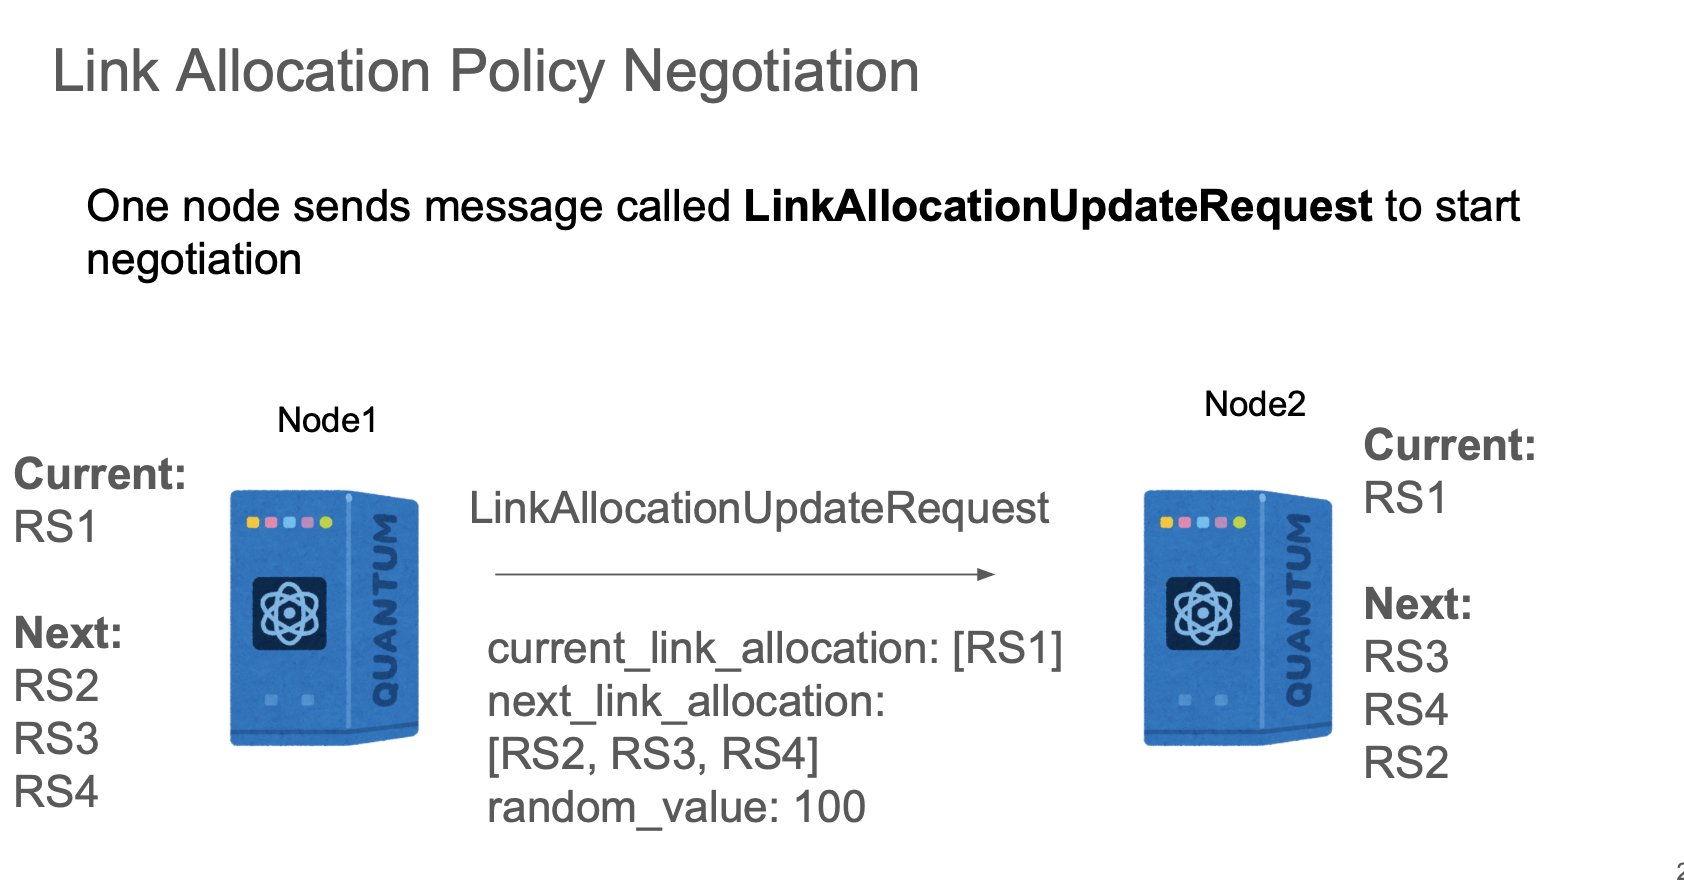
\includegraphics[width=.5\columnwidth]{images/link_allocation_update_message.png}}
  \caption{Transmission of a LinkAllocationUpdateMessage}
\end{figure}

First of all, LinkAllocationUpdateMessages are sent to all the neighboring nodes. Here is the pseudocode of the transmission of those messages.

\begin{algorithm}[H]
  \caption{Algorithm For Sending LinkAllocationUpdateMessages}
  \begin{algorithmic}[1]
  \Require The address of this node $parent\_address$
  \Require An array of available runtimes $runtimes$
  \Require A map of node address of each neighboring nodes and the active link allocation policy $node\_address\_active\_link\_allocations\_map$
  \Require A map of node address of each neighboring nodes and the next link allocation policy $node\_address\_next\_link\_allocations\_map$
  \Require A map of node address of each neighboring nodes and a random number $node\_address\_random\_number\_map$
  \Require A map of node address of each neighboring nodes and whether a LinkAllocationUpdateMessage is sent from this node $node\_address\_lau\_sent\_map$
  \Function {SendLinkAllocationUpdateMessages}{}
    \State Initialize an array of node addresses of neighboring nodes ${partner\_addresses}$
    \ForAll {$runtime \gets runtimes$} 
      \ForAll {$partner \gets$ the list of all the neighboring addresses that $runtime$ needs to communicate} 
      \State Append $partner$ to ${partner\_addresses}$ if it has not been added
      \EndFor
    \EndFor
    \ForAll {$runtime \gets runtimes$} 
      \ForAll {$partner \gets$ the list of all the neighboring addresses that $runtime$ needs to communicate} 
      \State Initialize an array for RuleSet IDs in the active link policy ${active\_link\_allocations}$
        \If {$partner$ is a part of the key of $node\_address\_active\_link\_allocations\_map$}
          \ForAll {$active\_link\_allocation \gets node\_address\_active\_link\_allocations\_map[partner]$}
            \State Append $active\_link\_allocation$ to ${active\_link\_allocations}$
          \EndFor
        \EndIf
      \State Initialize an array for RuleSet IDs in the next link policy ${next\_link\_allocations}$
        \If {$partner$ is a part of the key of $node\_address\_next\_link\_allocations\_map$}
          \ForAll {$next\_link\_allocation \gets node\_address\_next\_link\_allocations\_map[partner]$}
            \State Append $next\_link\_allocation$ to ${next\_link\_allocations}$
          \EndFor
        \EndIf
        \ForAll {$active\_link\_allocation \gets active\_link\_allocations$}
          \State{Append $active\_link\_allocation$ to $node\_address\_active\_link\_allocations\_map[partner]$}
        \EndFor
        \ForAll {$next\_link\_allocation \gets next\_link\_allocations$}
          \State{Append $next\_link\_allocation$ to $node\_address\_next\_link\_allocations\_map[partner]$}
        \EndFor
      \EndFor
      \algstore{hoge}
    \end{algorithmic}
  \end{algorithm}

  \begin{algorithm}[H]                   
    \begin{algorithmic}[1]
      \algrestore{hoge}
      \ForAll {$partner\_address \gets partner\_addresses$}
        \State Initialize an new LinkAllocationUpdateMessage $pkt$
        \State The source address of $pkt \gets parent\_address$ 
        \State The target address of $pkt \gets partner\_address$ 
        \ForAll {$active\_link\_allocation \gets node\_address\_active\_link\_allocations\_map[partner]$}
          \State Append $active\_link\_allocation$ to activeLinkAllocations of $pkt$
        \EndFor
        \ForAll {$next\_link\_allocation \gets node\_address\_next\_link\_allocations\_map[partner]$}
          \State Append $next\_link\_allocation$ to nextLinkAllocations of $pkt$
        \EndFor
        \State {Initialize a random integer $rand\_number$}
        \State The random number of $pkt \gets rand\_number$ 
        \State $node\_address\_random\_number\_map[partner\_address] \gets rand\_number$
        \State $node\_address\_lau\_sent\_map[partner\_address] \gets$ True
        \State Send $pkt$
      \EndFor
    \EndFor
  \EndFunction
  \end{algorithmic}
\end{algorithm}

If the RuleEngine receives an incoming LinkAllocationUpdateMessage, it has to store the information for the further negotiation.
\begin{algorithm}[H]  
  \caption{Algorithm For Storing the Information of an Incoming LinkAllocationUpdateMessage}                 
  \begin{algorithmic}[1]
    \Require An incoming LinkAllocationUpdateMessage $pkt$
    \Require  A map of node address of each neighboring nodes and the incoming random number $node\_address\_incoming\_random\_number\_map$
    \Require  A map of node address of each neighboring nodes and the incoming active link allocation policy $node\_address\_incoming\_active\_link\_allocations\_map$
    \Require  A map of node address of each neighboring nodes and the incoming next link allocation policy $node\_address\_incoming\_next\_link\_allocations\_map$
    \Require  A map of node address of each neighboring nodes and whether the RuleSet received LinkAllocationUpdateMessage $node\_address\_lau\_received\_map$
    \State $src\_addr \gets$ the source address of $pkt$
    \State $random\_number \gets the random number of pkt$
    \State $node\_address\_incoming\_random\_number\_map[src\_addr] \gets random\_number$
    \State $incoming\_active\_link\_allocations\_count \gets$ the number of RuleSets in the active link allocation policy
    \For{$i \gets 0$ to $incoming\_active\_link\_allocations\_count$}  
      \State $incoming\_active\_link\_allocation \gets$ $i$th element of the ActiveLinkAllocations of $pkt$
      \State Append $incoming\_active\_link\_allocation$ to $node\_address\_incoming\_active\_link\_allocations\_map[src_addr]$
    \EndFor
    \State $incoming\_next\_link\_allocations\_count \gets$ the number of RuleSets in the next link allocation policy
    \For{$i \gets 0$ to $incoming\_next\_link\_allocations\_count$}  
      \State $incoming\_next\_link\_allocation \gets$ $i$th element of the NextLinkAllocations of $pkt$
      \State Append $incoming\_next\_link\_allocation$ to $node\_address\_incoming\_next\_link\_allocations\_map[src_addr]$
    \EndFor
    \State $node\_address\_lau\_received\_map[src\_addr] \gets$ True
  \end{algorithmic}
\end{algorithm}

After exchanging LinkAllocationUpdateMessages, each pair of nodes need to synchronize the contents and their order of the next link allocation policy.
The policy from the LinkAllocationUpdateMessage with the bigger random value will be prioritized.

\begin{algorithm}[H]  
  \caption{Algorithm For Synchronizing the Link Allocation Policy}                 
  \begin{algorithmic}[1]
    \Require The address of the destination node $dest\_address$
    \Require A map of node address of each neighboring nodes and the incoming random number $node\_address\_incoming\_random\_number\_map$
    \Require A map of node address of each neighboring nodes and the random number in this node $node\_address\_random\_number\_map$
    \Require  A map of node address of each neighboring nodes and the incoming next link allocation policy $node\_address\_incoming\_next\_link\_allocations\_map$
    \Require  A map of node address of each neighboring nodes and the next link allocation policy in this node $node\_address\_next\_link\_allocations\_map$
    \Require  A map of node address of each neighboring nodes and whether the RuleSet sent BarrierMessage $node\_address\_barrier\_sent\_map$
    \Require  A map of node address of each neighboring nodes and whether the RuleSet received BarrierMessage $node\_address\_barrier\_received\_map$
    \State $incoming\_random\_number \gets node\_address\_incoming\_random\_number\_map[dest\_address]$
    \State $random\_number \gets node\_address\_random\_number\_map[dest\_address]$
    \If{$incoming\_random\_number > random\_number$}
      \State $node\_address\_incoming\_random\_number\_map[dest\_address] \gets node\_address\_random\_number\_map[dest\_address]$
    \EndIf
    \State $node\_address\_barrier\_sent\_map[src\_addr] \gets$ True
    \State $node\_address\_barrier\_received\_map[src\_addr] \gets$ True
  \end{algorithmic}
\end{algorithm}

\subsubsection{Link Allocation Timing Negotiation}

After the next link allocation policy is synchronized between two neighboring nodes, it is time to determine when to update the link allocation policy.
\begin{algorithm}[H]  
  \caption{Algorithm For Sending a BarrierMessage}             
  \begin{algorithmic}[1]
    \Require The address of the this node $this\_address$      
    \Require The address of the destination node $dest\_address$    
    \State Initialize a new BarrierRequest $pkt$
    \State The source address of $pkt \gets this\_address$
    \State The destination address of $pkt \gets dest\_address$
    \State $sequence\_number \gets$ the smallest value among sequence numbers of the available link Bell pairs
    \State The sequence number of $pkt \gets sequence\_number$
    \State Send $pkt$
  \end{algorithmic}
\end{algorithm}

\begin{algorithm}[H]  
  \caption{Algorithm For Storing Information About the Incoming BarrierMessage}                 
  \begin{algorithmic}[1]
    \Require The incoming BarrierMessage $pkt$
    \Require A map of node address of each neighboring nodes and the smallest sequence number in this node $node\_address\_barrier\_sequence\_number\_map$
    \Require A map of node address of each neighboring nodes and whether the RuleSet received BarrierMessage $node\_address\_barrier\_received\_map$
    \State $sequence\_number \gets$ the smallest value among sequence numbers of the available link Bell pairs
    \State $node\_address\_incoming\_sequence\_number\_map[src\_addr] \gets sequence\_number$
  \end{algorithmic}
\end{algorithm}

\begin{algorithm}[H]  
  \caption{Algorithm For Synchronizing the Next Sequence Number}                 
  \begin{algorithmic}[1]
    \Require The node address of one of the neighboring nodes $src\_address$
    \Require A map of node address of each neighboring nodes and the smallest sequence number in this node $node\_address\_sequence\_number\_map$
    \Require A map of node address of each neighboring nodes and the incoming smallest sequence number $node\_address\_incoming\_sequence\_number\_map$
    \State $sequence\_number \gets node\_address\_sequence\_number\_map[src\_address]$
    \State $incoming\_sequence\_number \gets node\_address\_incoming\_sequence\_number\_map[src\_address]$
    \If {$incoming\_sequence\_number > sequence\_number$}
      \State $node\_address\_sequence\_number\_map[src\_addr] \gets incoming\_sequence\_number$
    \EndIf
  \end{algorithmic}
\end{algorithm}

\subsubsection{Link Management in QuISP}

Allocation of link Bell pairs starts after two neighboring nodes coordinates the first sequence number to start applying the new link allocation policy.

\begin{algorithm}[H]  
  \caption{Algorithm For Allocating Link Bell pairs}                 
  \begin{algorithmic}[1]
    \State Initialize a map of node addresses of neighboring nodes and the indices of Runtimes $partner\_addr\_runtime\_indices\_map$
    \State $index \gets$ 0
    \ForAll {$runtime \gets runtimes$}
      \State $partners \gets$ the addresses of all nodes that $runtime$ needs to communicate
      \ForAll {$partner \gets partners$} 
        \State Append $partner$ to $partner\_addr\_runtime\_indices\_map[partner]$
      \EndFor
      \State $index \gets index + 1$
    \EndFor

    \ForAll {$[partner\_addr, value] \gets partner\_addr\_runtime\_indices\_map$}
      \State $runtime\_indices \gets partner\_addr\_runtime\_indices\_map[partner_addr]$
      \State $bell\_pair\_range \gets$ the list of Bell pairs on the side of this node
      \State $bell\_pair\_num \gets$ 0
      \ForAll {$bell\_pair \gets bell\_pair\_range$}
        \State $bell\_pair\_num \gets bell\_pair\_num + 1$
      \EndFor

      \State  Initialize a map of Runtime indices and the number of Bell pairs $runtime\_index\_bell\_pair\_number\_map$
      \State 

    \EndFor
    \State $number \gets$ 0

  \end{algorithmic}
\end{algorithm}


\subsection{Relationship with Connection Management}
\subsubsection{Connection Setup}
\subsubsection{Connection Teardown}


%%% Local Variables:
%%% mode: japanese-latex
%%% TeX-master: "../bthesis"
%%% End:
